\chapter{Confronto tra le implementazioni}
Nel corso degli ultimi anni la community di sviluppatori ha portato avanti diverse iniziative per imporre uno standard condiviso per le STOs. Inizialmente lo standard de facto è stato \textit{ERC-20}\cite{K37}, già ampiamente adottato dalla maggior parte delle ICOs. Tra gli standard utilizzati per le STOs, ERC-20 è lo standard più maturo e con maggiore supporto essendo stato creato verso la fine del 2015. Altri tentativi di standardizzazione nascono dalla necessità di garantire all'issuer della STO una maggiore governance e per facilitare il rispetto delle regolamentazioni sulle securities. Non a caso possiamo osservare come molti tentativi di standardizzazione siano stati operati da aziende che offrono piattaforme per l'emissione di tokens. Per la maggior parte di queste aziende l'approccio è stato quello di estendere lo standard ERC-20, in modo da ottenere retrocompatibilità ed essere più appetibili alla community di sviluppatori con conoscenza dello standard sopracitato. Tra i casi che verranno analizzati troviamo: 
\begin{itemize}
    \item \textit{ST-20}, sviluppato da Polymath
    \item \textit{R-Token}, sviluppato da Harbor
    \item \textit{DS Protocol}, sviluppato da Securitize
    \item \textit{T-REX}, sviluppato da Tokeny
    \item \textit{S3}, sviluppato da OpenFinace
\end{itemize}

Altri standard si sono sviluppati a partire da necessità diverse, come nel caso degli standard \textit{ERC-721} ed \textit{ERC-1155} che implementano tokens non fungibili. La notorietà di questi protocolli è in parte dovuta all'introduzione del concetto di scarsità digitale tramite l'utilizzo di tokens non omogenei, un approccio che ben si presta all'ambito videoludico. 
Una proposta più recente e che ha ottenuto maggiore supporto sia dalla community sia da aziende, alcune delle quali già in possesso di uno standard proprietario, è lo standard \textit{ERC-1400}, rinominato \textit{Security Token Standard}. ERC-1400 è una collezione di diversi standard sviluppati per essere interoperabili e facilmente estendibili all'emergere della necessità di nuove funzionalità da introdurre. Il passaggio ad uno standard condiviso e supportato da più stakeholder rappresenta uno step fondamentale par la diffusione di questo fenomeno.

\section{Implementazione con token ERC-20}
ERC-20 definisce un'interfaccia standard che rappresenta un token. Lo standard fornice funzionalità basilari per il trasferimento dei tokens. Lo scopo principale dello standard è quello di permettere interoperabilità tra le applicazioni che supportano lo standard, come ad esempio wallets ed exchanges. 
Lo standard ERC-20 prevede le seguenti funzioni:
\begin{lstlisting}[language=Solidity,numbers=none]
totalSupply() public view returns (uint256 totalSupply)
\end{lstlisting} 
\begin{lstlisting}[language=Solidity,numbers=none]
balanceOf(address _owner) public view returns (uint256 balance)\end{lstlisting}
\begin{lstlisting}[language=Solidity,numbers=none] 
transfer(address _to, uint256 _value) public returns (bool success)\end{lstlisting} 
\begin{lstlisting}[language=Solidity,numbers=none]
transferFrom(address _from, address _to, uint256 _value) public returns (bool success)
\end{lstlisting}
\begin{lstlisting}[language=Solidity,numbers=none]
approve(address _spender, uint256 _value) public returns (bool success)
\end{lstlisting}
\begin{lstlisting}[language=Solidity,numbers=none]
allowance(address _owner, address _spender) public view returns (uint256 remaining)
\end{lstlisting}
Inoltre, vengono definiti i seguenti eventi:
\begin{lstlisting}[language=Solidity,numbers=none]
Transfer(address indexed _from, address indexed _to, uint256 _value)
\end{lstlisting}
\begin{lstlisting}[language=Solidity,numbers=none]
Approval(address indexed _owner, address indexed _spender, uint256 _value)
\end{lstlisting}
Due delle implementazioni più diffuse di questo standard sono state realizzate da OpenZeppelin e ConsenSys. Le due implementazioni sono entrambe pienamente compatibili con lo standard sebbene presentino delle lievi differenze come si può osservare in appendice \ref{appendix:ERC-20Interface}.

Una appunto interessante si può trarre osservando i cambiamenti avvenuti durante lo sviluppo iniziale dello standard. Se in principio le prime bozze dello standard prevedevano un focus sulla creazione di \textit{‘‘Coins’’}, gli sviluppatori in modo lungimirante hanno deciso di generalizzare il protocollo per renderlo applicabile ad ogni bene fungibile trasferibile, motivo per il quale è stata scelta la denominazione più generica di \textit{‘‘token’’}.

\subsection{ERC-20 proprietary extension}
\subsubsection{ST-20}
Lo standard ST-20, introdotto da Polymath, nasce con l'obbiettivo di aggiungere all'interfaccia ERC20 la possibilità di inserire restrizioni allo scambio di tokens in modo da poter essere conforme alle normative sulle securities. 
In appendice \ref{appendix:ST20} è possibile osservare l'interfaccia dello smart contract che definisce un security token che rispetta lo standard ST-20. Trattandosi di un'estensione, lo smart contract è compatibile con lo standard ERC-20 e ne implementa tutte le funzioni e gli eventi previsti, aggiungendo a questi altre funzionalità e caratteristiche che agevolano l'adattabilità e la governance della STO. Per esempio, nel caso dello scambio senza restrizioni tra due parti, un caso che non sempre è desiderabile nelle STOs, le transazioni possono essere limitare da una funzione \textit{‘‘verifyTransfer’’}. Ciò permette inoltre l'implementazione di una whitelist, una blacklist, un limite minimo/massimo di trasferimento, etc. 
In modo più dettagliato, l'interfaccia creata da Polymath si avvale principalmente di tre tipi componenti: un primo tipo detto \textit{‘‘Transfer Manager’’}, un tipo di moduli denominati \textit{‘‘permission modules’’} e infine un modulo che si occupa delle funzionalità della token sale, ovvero \textit{‘‘STO module’’}. 
L'utilizzo di numerose componenti per implementare diverse funzionalità permette di avere un architettura modulare che comprende di volta in volta solamente le funzionalità richieste, permettendo così di rendere lo smart contract più efficiente.

\subsubsection{R-Token}
R-token, implementato da Harbor, offre delle caratteristiche che lo rendono particolarmente innovativo, tanto da essere concettualmente compatibile con un token ERC-1400. Un altro aspetto particolare del protocollo è l'integrazione di una whitelist per gli operatori presenti nell'ecosistema proposto da Harbor. 
R-Token, che sta per \textit{‘‘regualted token’’} si differenzia dagli altri standard compatibili con ERC-20 per l'adozione di alcuni servizi di document management e di custody. 
Generalmente una STO Harbor si compone di tre smart contracts:
\begin{itemize}
    \item Un \textit{‘‘Regulator Service’’} che si occupa di interagire tramite un oracolo con la regolamentazione definita off-chain. 
    \item Un \textit{‘‘Service Registry’’} che contiene un riferimento al \textit{‘‘Regulator Service’’}. Questo riferimento può essere modificato per permettere di aggiornare la business logic della STO. 
    \item Uno smart contract \textit{‘‘R-Token’’} che contiene le caratteristiche del token, le sue funzioni e un riferimento immutabile al \textit{‘‘Service Registry’’}.
\end{itemize}
\subsubsection{DS Protocol}
L'estensione di ERC-20, proposta da Securitize, ha due componenti principali. Il primo è lo smart contract \textit{‘‘DSTokenInterface’’} che nel complesso non risulta apportare cambiamenti rilevanti rispetto ai protocolli già presentati. Il secondo componente risulta essere più originale ed è lo smart contract \textit{‘‘DSServiceConsumerInterface’’} definito come segue:
\begin{lstlisting}[language=Solidity,numbers=none]
function getDSService(uint _serviceId) public view returns (address);

function setDSService(uint _serviceId, address _address) public /*onlyMaster*/ returns (bool);
\end{lstlisting}
Queste funzioni permettono l'associazione dinamica di componenti e di verificare la presenza componenti  in modo dinamico (al fine di mantenere compatibilità tra diverse versioni del protocollo). I servizi sono identificati da un id nel seguente modo:
\begin{lstlisting}[language=Solidity,numbers=none]
 uint public constant TRUST_SERVICE = 1;
 uint public constant DS_TOKEN = 2;
 uint public constant REGISTRY_SERVICE = 4;
 uint public constant COMPLIANCE_SERVICE = 8;
 uint public constant COMMS_SERVICE = 16;
 uint public constant WALLET_MANAGER = 32;
 uint public constant LOCK_MANAGER = 64;
 uint public constant ISSUANCE_INFORMATION_MANAGER = 128;
 \end{lstlisting}
\subsubsection{T-REX}
T-REX, per esteso \textit{‘‘Token for Regulated EXchanges’’}, presenta un approccio diverso rispetto ad altri protocolli. L'identità, infatti, ricopre un ruolo fondamentale nel protocollo, tanto da prevedere dei meccanismi di gestione dell'identità dell'investitore on-chain secondo i protocolli \textit{ERC-725} ed \textit{ERC-735}. Il meccanismo di controllo dell'identità sostituisce la logica di whitelisting e blacklisting rendendo il protocollo più flessibile. Possiamo osservare il funzionamento del protocollo nel seguente diagramma in figura \ref{fig:trex}.
\begin{figure}[H]
  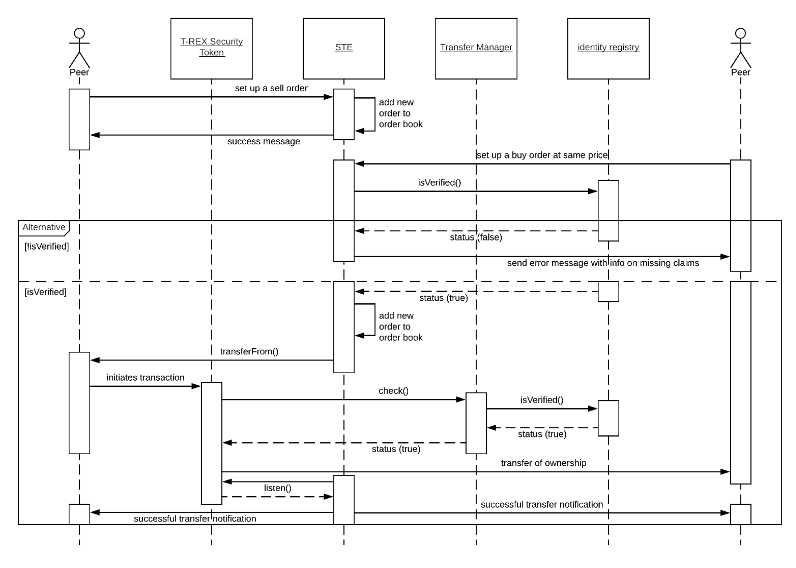
\includegraphics[width=\linewidth]{trex.png}
  \caption{Sequence diagram of a Distributed Security Token Exchange  transaction with T-REX tokens}
  \label{fig:trex}
\end{figure}
\subsubsection{S3}
S3, per esteso \textit{‘‘Smart Securities Standard’’}, è un altra estensione di ERC-20 che si distingue per una semplice caratteristica di compliance poiché il protocollo S3 include degli smart contracts dedicati ad implementare le restrizioni e le regole imposte dalla \textit{Regulation D}, la \textit{Regulation S}, la \textit{Regulation A+} e \textit{Regulation CF}.

\begin{lstlisting}[language=Solidity,numbers=none]
///RegD506c.sol
/// @title Functions that tokens will need to call to configure themselves 
contract RegD506c is TransferRestrictor {
  function startHoldingPeriod() public;
  function registerAmlKycChecker(address _checker, address _token) public;
  function registerAccreditationChecker(address _checker, address _token) public;
}
\end{lstlisting}

Questo approccio semplifica notevolmente la struttura del protocollo ma presenta numerosi svantaggi, soprattutto in termini di manutenibilità. Nell'ultima versione disponibile del protocollo l'approccio è mutato notevolmente, tanto che la restrizione degli scambi è delegata ad un altro smart contract non specificato. 
\section{Implementazione con token ERC-721 e ERC-1155}
Sebbene non siano pensati in modo specifico per le securities, gli standard ERC-721 ed ERC-1155 sono rilevanti per l'argomento analizzato in quanto permettono di tokenizzare assets fisici. Tramite l'introduzione del concetto di non fungibilità nello standard ERC-721 è possibile definire uno smart contract in cui un token è unico. Questo concetto si può applicare con facilità ad oggetti rari, unici oppure ogni tipo di oggetto collezionabile. La sua implementazione più famosa è il progetto \textit{CryptoKitties}, un gioco che permette di comprare, vendere e scambiare carte virtuali. nel 2017 il gioco divenne talmente popolare da congestionare la rete Ethereum. Ogni carta rappresenta un \textit{CryptoKitty}, ovvero un token  non-fungibile. Ad oggi sono stati scambiati CryptoKitties per un valore superiore a 27 milioni di dollari. Il valore di un singolo token può raggiungere cifre molto alte e sono nati exchanges dedicati a questo protocollo, come possiamo vedere in figura \ref{fig:kitty}: un singolo token, associato a questo CryptoKitty, è stato venduto per 253 ethers, ovvero 114mila dollari. 
\begin{figure}[H]
  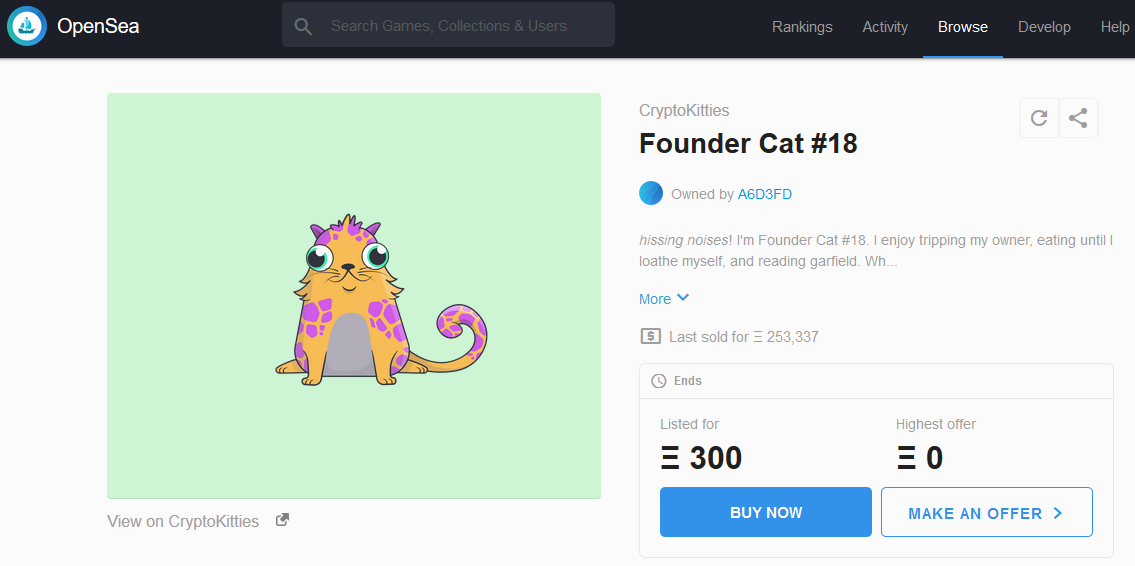
\includegraphics[width=\linewidth]{kitty.png}
  \caption{Second most expensive CryptoKitty, traded on a specialized exchange}
  \label{fig:kitty}
\end{figure}

ERC-1155 rappresenta un evoluzione dei tokens ERC-20 ed ERC-721, poiché permette di gestire sia tokens fungibili che non fungibili in un unico contratto, permettendo transazioni con più tokens di tipo diverso. Questa funzionalità è stata realizzata con l'obbiettivo di permettere l'adozione di tokens in videogiochi più complessi rispetto a CryptoKitties, come nel caso di giochi che permetto la vendita, l'acquisto e lo scambio di una currency del gioco e di oggetti virtuali. 

\section{Implementazione con token ERC-1400}
Lo standard ERC-1400 è nato in seguito allo sforzo di numerosi operatori del settore per cercare di ottenere uno standard condiviso. Grazie all'ampio supporto ricevuto da queste aziende, alcune delle quali già promotrici di standard illustrati in precedenza, ERC-1400 si sta affermando come uno standard \textit{de facto} per la creazione di STOs.
Inizialmente ERC-1400 è stato pensato come uno standard per realizzare security tokens ma già dalle prime fasi di sviluppo è emersa la necessità di definire un protocollo modulare e facilmente espandibile. Proprio per questo, ERC-1400 è una collezione di standard interoperabili. Lo sviluppo di ERC-1400 non segue una roadmap definita in quanto lo scopo degli autori è quello di aggiungere il supporto di nuove funzionalità qualora gli utilizzatori ne esprimano il bisogno. Nonostante la mancanza di una roadmap, gli autori hanno informalmente assicurato nuove release approssimativamente ogni sei mesi, questo per facilitare l'adozione da parte delle aziende interessate.  
Grazie alla discussione tra più gruppi e al contributo di più aziende, lo standard copre la maggior parte degli scenari che possono presentarsi in una STO. Ad esempio, nella figura \ref{fig:1400} possiamo vedere come siano stati dedicati diversi codici di errore a varie situazioni, un notevole miglioramento nell'aspetto di governance rispetto allo standard ERC-20. 
\begin{figure}[H]
  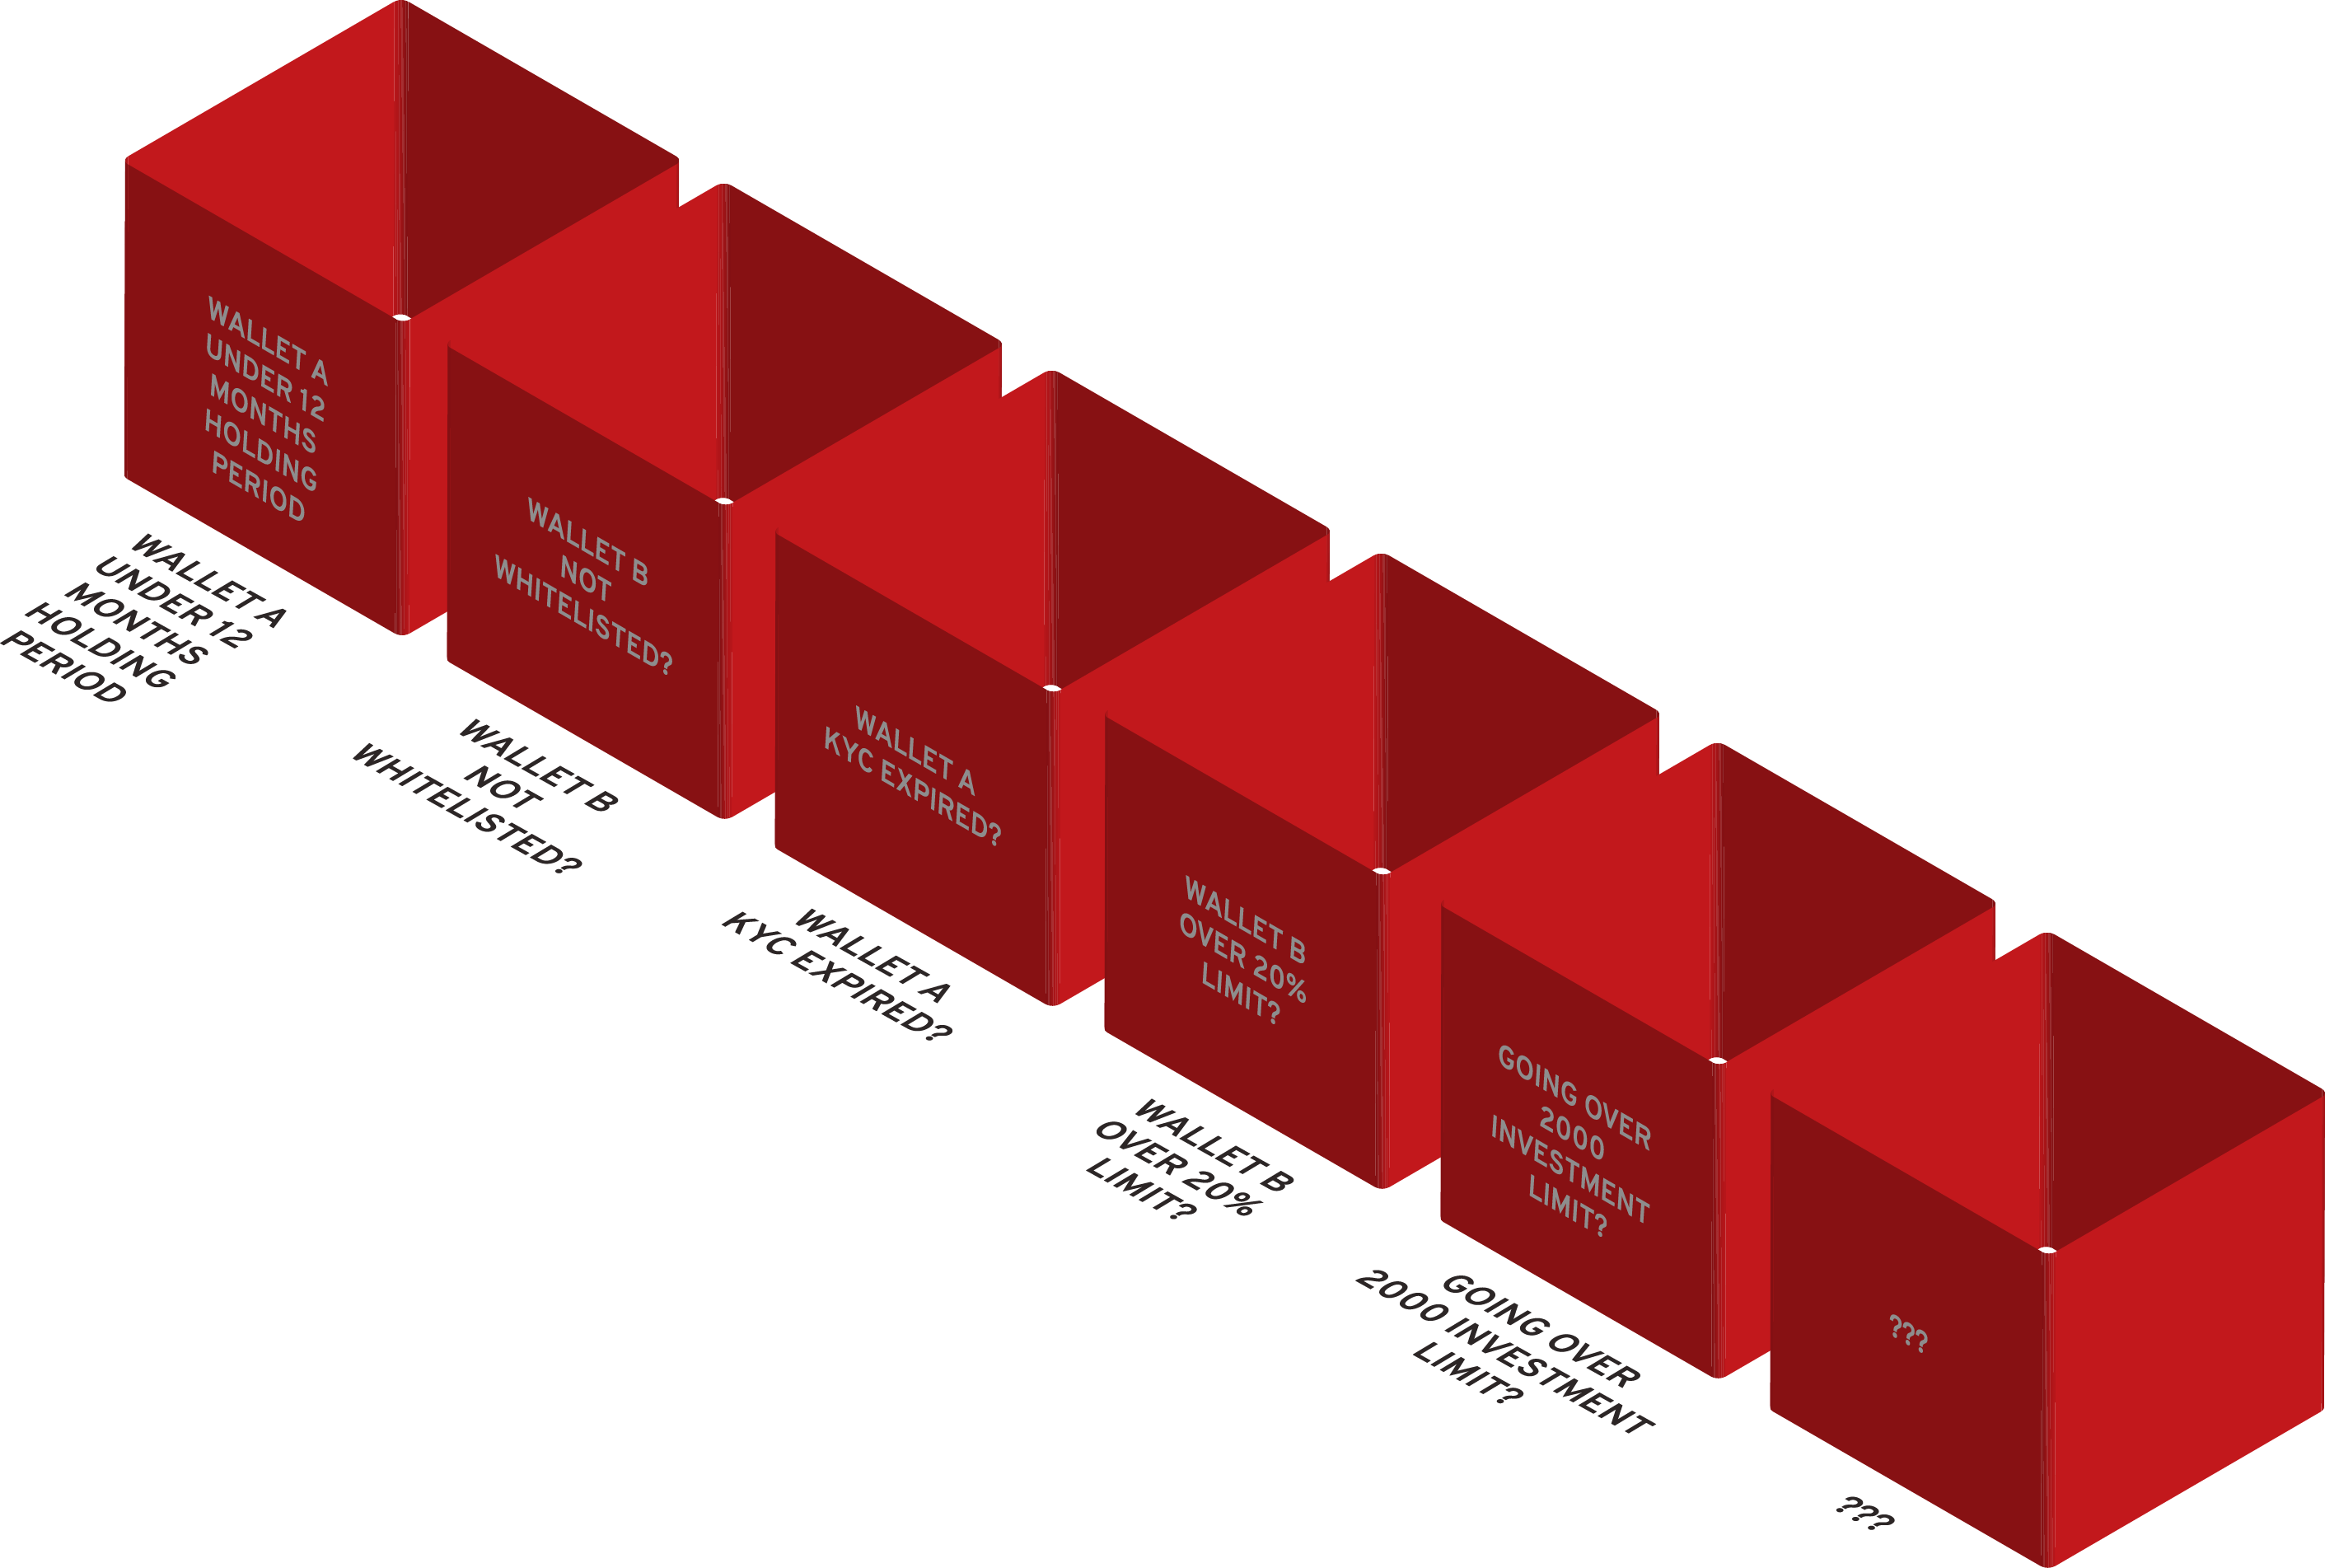
\includegraphics[width=\linewidth]{1400.png}
  \caption{ERC-1400 Error cases examples}
  \label{fig:1400}
\end{figure}

La collezione di standard definiti da ERC-1400 ad oggi fornisce funzionalità di gestione della documentazione, gestione degli errori, controllo delle transazioni, input di dati off-chain, gestione dell'emissione dei tokens e differenziazione dei tokens. 
Analizzare nel dettaglio queste features risulta agevole grazie alla modularità dello standard. Al momento, ERC-1400 comprende i seguenti standard:
\begin{itemize}
    \item ERC-1410
    \item ERC-1594
    \item ERC-1643
    \item ERC-1644
    \item ERC-2258 \textit{(in fase di adozione)}
\end{itemize}

\subsection{ERC-1410: Partially Fungible Token Standard}
Il primo standard previsto da ERC-1400 è lo standard ERC-1410, che riguarda l'introduzione del concetto di fungibilità parziale. Oltre ad essere il primo standard introdotto è anche il più corposo poiché aggiunge un meccanismo di partizioni per ottenere non fungibilità parziale. All'interno di ogni partizione ogni tokens è fungibile ma tokens di partizioni diverse sono non fungibili tra loro.   

\begin{lstlisting}[language=Solidity,numbers=none]
/// @title ERC-1410 Partially Fungible Token Standard
/// @dev See https://github.com/SecurityTokenStandard/EIP-Spec

interface IERC1410 {

    // Token Information
    function balanceOf(address _tokenHolder) external view returns (uint256);
    function balanceOfByPartition(bytes32 _partition, address _tokenHolder) external view returns (uint256);
    function partitionsOf(address _tokenHolder) external view returns (bytes32[]);
    function totalSupply() external view returns (uint256);

    // Token Transfers
    function transferByPartition(bytes32 _partition, address _to, uint256 _value, bytes _data) external returns (bytes32);
    function operatorTransferByPartition(bytes32 _partition, address _from, address _to, uint256 _value, bytes _data, bytes _operatorData) external returns (bytes32);
    function canTransferByPartition(address _from, address _to, bytes32 _partition, uint256 _value, bytes _data) external view returns (byte, bytes32, bytes32);    

    // Operator Information
    function isOperator(address _operator, address _tokenHolder) external view returns (bool);
    function isOperatorForPartition(bytes32 _partition, address _operator, address _tokenHolder) external view returns (bool);

    // Operator Management
    function authorizeOperator(address _operator) external;
    function revokeOperator(address _operator) external;
    function authorizeOperatorByPartition(bytes32 _partition, address _operator) external;
    function revokeOperatorByPartition(bytes32 _partition, address _operator) external;

    // Issuance / Redemption
    function issueByPartition(bytes32 _partition, address _tokenHolder, uint256 _value, bytes _data) external;
    function redeemByPartition(bytes32 _partition, uint256 _value, bytes _data) external;
    function operatorRedeemByPartition(bytes32 _partition, address _tokenHolder, uint256 _value, bytes _operatorData) external;

    // Transfer Events
    event TransferByPartition(
        bytes32 indexed _fromPartition,
        address _operator,
        address indexed _from,
        address indexed _to,
        uint256 _value,
        bytes _data,
        bytes _operatorData
    );

    // Operator Events
    event AuthorizedOperator(address indexed operator, address indexed tokenHolder);
    event RevokedOperator(address indexed operator, address indexed tokenHolder);
    event AuthorizedOperatorByPartition(bytes32 indexed partition, address indexed operator, address indexed tokenHolder);
    event RevokedOperatorByPartition(bytes32 indexed partition, address indexed operator, address indexed tokenHolder);

    // Issuance / Redemption Events
    event IssuedByPartition(bytes32 indexed partition, address indexed operator, address indexed to, uint256 amount, bytes data, bytes operatorData);
    event RedeemedByPartition(bytes32 indexed partition, address indexed operator, address indexed from, uint256 amount, bytes operatorData);

}
\end{lstlisting}

Ogni partizione è identificata da una chiave e dei metadati arbitrari. Ogni token contiene le informazioni sulla partizione a cui appartiene. 
Questo meccanismo di partizioni risulta utile per identificare e distinguere tokens che hanno restrizioni o benefici diversi. Infatti, questa funzionalità permette di distinguere i tokens in base alla fase della token sale in cui sono stati generati per permettere il \textit{vesting} dei tokens oppure per determinare differenti capacità di voto legate al possesso del token. 

\subsection{ERC-1594: Core Security Token Standard}
Questo standard permette l'esecuzione di operazioni che includono l'iterazione tra dati on-chain e off-chain. Fornire dati off-chain permette ad esempio di eseguire una operazioni autorizzate off-chain con una firma, senza dover ricorrere ad una whitelist on-chain. Questo protocollo si occupa anche di verificare la possibilità di eseguire un operazione e restituire un appropriato \textit{status code} di risposta, evitando di dover provare ad eseguire l'operazione per poi vederla fallire. 
Infine, in questo standard vengono incorporate le funzionalità di gestione della token sale, in particolare con le funzioni relative all'emissione e alla riscossione. 

\begin{lstlisting}[language=Solidity,numbers=none]
/// @title IERC1594 Security Token Standard
/// @dev See https://github.com/SecurityTokenStandard/EIP-Spec

interface IERC1594 is IERC20 {

    // Transfers
    function transferWithData(address _to, uint256 _value, bytes _data) external;
    function transferFromWithData(address _from, address _to, uint256 _value, bytes _data) external;

    // Token Issuance
    function isIssuable() external view returns (bool);
    function issue(address _tokenHolder, uint256 _value, bytes _data) external;

    // Token Redemption
    function redeem(uint256 _value, bytes _data) external;
    function redeemFrom(address _tokenHolder, uint256 _value, bytes _data) external;

    // Transfer Validity
    function canTransfer(address _to, uint256 _value, bytes _data) external view returns (bool, byte, bytes32);
    function canTransferFrom(address _from, address _to, uint256 _value, bytes _data) external view returns (bool, byte, bytes32);

    // Issuance / Redemption Events
    event Issued(address indexed _operator, address indexed _to, uint256 _value, bytes _data);
    event Redeemed(address indexed _operator, address indexed _from, uint256 _value, bytes _data);

}
\end{lstlisting}


\subsection{ERC-1643: Document Management Standard}
Questo standard permette di collegare dei documenti ad uno smart contract ed offre la possibilità di aggiornarli. I documenti possono essere per esempio prospetti informativi sulla security ed in generale qualsiasi documento legale necessario.
\begin{lstlisting}[language=Solidity,numbers=none]
/// @title IERC1643 Document Management (part of the ERC1400 Security Token Standards)
/// @dev See https://github.com/SecurityTokenStandard/EIP-Spec

interface IERC1643 {

    // Document Management
    function getDocument(bytes32 _name) external view returns (string, bytes32, uint256);
    function setDocument(bytes32 _name, string _uri, bytes32 _documentHash) external;
    function removeDocument(bytes32 _name) external;
    function getAllDocuments() external view returns (bytes32[]);

    // Document Events
    event DocumentRemoved(bytes32 indexed _name, string _uri, bytes32 _documentHash);
    event DocumentUpdated(bytes32 indexed _name, string _uri, bytes32 _documentHash);

}
\end{lstlisting}
Una lieve criticità di questo standard è la gestione di documenti privati. Ciò avviene poiché lo standard rende possibili solo due alternative per gestire questo caso d'uso: rendere pubblico il documento privato oppure imporre una password per accedere al documento (dovendo quindi fornire una password all'interessato tramite un canale di comunicazione esterno). Al momento, non essendo presenti alternative valide, il metodo preferibile è il secondo. 

\subsection{ERC-1644: Controller Token Operation Standard}
Questo standard permette di eseguire operazioni di trasferimento forzato dei tokens. Poiché soggetti a regolamentazioni diverse in base alla giurisdizione, in alcuni casi i security tokens devono poter essere trasferiti forzatamente. Questa situazione si presenta nel caso in cui ci sia necessità di annullare una transazione fraudolenta o per rispondere ad ordini del tribunale. Vista la sensibilità di questa operazione solo un indirizzo autorizzato ha i permessi per eseguirla:

\begin{lstlisting}[language=Solidity,numbers=none]
/// @title IERC1644 Controller Token Operation (part of the ERC1400 Security Token Standards)
/// @dev See https://github.com/SecurityTokenStandard/EIP-Spec

interface IERC1644 is IERC20 {

    // Controller Operation
    function isControllable() external view returns (bool);
    function controllerTransfer(address _from, address _to, uint256 _value, bytes _data, bytes _operatorData) external;
    function controllerRedeem(address _tokenHolder, uint256 _value, bytes _data, bytes _operatorData) external;

    // Controller Events
    event ControllerTransfer(
        address _controller,
        address indexed _from,
        address indexed _to,
        uint256 _value,
        bytes _data,
        bytes _operatorData
    );

    event ControllerRedemption(
        address _controller,
        address indexed _tokenHolder,
        uint256 _value,
        bytes _data,
        bytes _operatorData
    );

}
\end{lstlisting}

Dato il contrasto tra questa funzionalità (necessaria per motivi di compliance) e i principi di decentralizzazione della blockchain, questa operazione deve svolgersi in modo trasparente. L'unico modo per garantire questa trasparenza è un protocollo dedicato che rende chiara la distinzione tra un trasferimento ed un trasferimento forzato. 

\subsection{ERC-2258: Custodial Ownership Standard}
Dato che un security token rappresenta un modo per registrare la proprietà di un asset sottostante, lo standard ERC-2258 è stato creato per soddisfare alcuni casi d'uso in cui il concetto di proprietà non è più sufficiente. Questo è il caso della custodia di un token da parte di un entità terza per conto del proprietario del token. In questo caso la proprietà del token non varia. Un esempio che rende più chiaro il meccanismo di funzionamento di questo standard è la necessità di utilizzare un security token come collaterale. Il proprietario deve poter continuare a beneficiare dei dividendi o del diritto di voto permessi dal token ma, allo stesso tempo, il custode deve poter trasferire la proprietà del token ad un altro beneficiario in caso di liquidazione della posizione.   
A seguire, possiamo osservare come le funzioni esposte dall'interfaccia dello standard abbiano lo scopo di definire le operazioni eseguibili da un custode: 
\begin{lstlisting}[language=Solidity,numbers=none]
/// @title IERCx Custodial Ownership Standard (part of the ERC1400 Security Token Standards Library)
/// @dev See https://github.com/SecurityTokenStandard/EIP-Spec

interface IERCx {

    // Increase the custody limit of a custodian either directly or via signed authorisation
    function increaseCustodyAllowance(address _custodian, uint256 _amount) external;
    function increaseCustodyAllowanceOf(address _tokenHolder, address _custodian, uint256 _amount, uint256 _nonce, bytes _sig) external;

    // Query individual custody limit and total custody limit across all custodians
    function custodyAllowance(address _tokenHolder, address _custodian) external view returns (uint256);
    function totalCustodyAllowance(address _tokenHolder) external view returns (uint256);

    // Allows a custodian to exercise their right to transfer custodied tokens
    function transferByCustodian(address _tokenHolder, address _receiver, uint256 _amount) external;

    // Custody Events
    event CustodyTransfer(address _custodian, address _from, address _to, uint256 _amount);
    event CustodyAllowanceChanged(address _tokenHolder, address _custodian, uint256 _oldAllowance, uint256 _newAllowance);

}
\end{lstlisting}

Lo standard permette al proprietario di nominare un custode e di affidargli un numero definito di tokens. 
Un altro motivo rilevante per l'introduzione del concetto di custodia è favorire la riduzione del rischio di frodi e di hacking grazie alla specializzazione di servizi dedicati. Ciò permette di evitare al proprietario del token l'onere di questi compiti.
